\documentclass[12pt]{article}
\usepackage[utf8]{inputenc}
\usepackage[spanish]{babel}
\shorthandoff{"}
\usepackage{csquotes}
\usepackage{tikz}
\usetikzlibrary{arrows.meta,positioning,shapes.geometric,babel}
\usepackage{amsmath}
\usepackage{eso-pic}
\usepackage{mathpazo} 
\usepackage{setspace}
\setstretch{1.2}
\setlength{\parskip}{10pt}
\usepackage{indentfirst}
\usepackage{geometry}
\usepackage{graphicx}
\usepackage{titlesec}
\usepackage{fancyhdr}
\usepackage{lipsum}
\usepackage{amsmath,bm}
\usepackage[utf8]{inputenc}
\usepackage[T1]{fontenc}
\usepackage{minted}
\usepackage{ragged2e}
\usepackage{hyperref}
\usepackage{amsthm}
\newtheorem{teorema}{Teorema}
\hypersetup{
    hidelinks
}
\usepackage{subcaption}
\usepackage{mfirstuc}
\usepackage{appendix}
\usepackage{titletoc}
\usepackage[style=apa,backend=biber,sorting=none]{biblatex}
\addbibresource{export.bib}
\usepackage{listings}
\usepackage{xcolor}

\graphicspath{{./figuras/}}

\geometry{
    top=2.54cm,
    left=2.54cm,
    right=2.54cm,
    bottom=2.54cm
}

\pagestyle{fancy}

\lhead{} \chead{} \rhead{\thepage}

\renewcommand{\headrulewidth}{0pt}

\lfoot{} \cfoot{} \rfoot{}

\renewcommand{\footrulewidth}{0pt}

\fancypagestyle{plain}{%
  \fancyhf{}%
  \renewcommand{\headrulewidth}{0pt}%
  \renewcommand{\footrulewidth}{0pt}%
}

% Configuración de estilo para el código MATLAB
\lstset{
    language=Matlab,
    basicstyle=\ttfamily\small,
    keywordstyle=\color{blue}\bfseries,
    commentstyle=\color{green!60!black},
    stringstyle=\color{purple},
    numbers=left,
    numberstyle=\tiny\color{gray},
    breaklines=true,
    frame=single,
    captionpos=b,
    showstringspaces=false,
    extendedchars=true,
literate=%
    {á}{{\'a}}1 {é}{{\'e}}1 {í}{{\'i}}1 {ó}{{\'o}}1 {ú}{{\'u}}1
    {Á}{{\'A}}1 {É}{{\'E}}1 {Í}{{\'I}}1 {Ó}{{\'O}}1 {Ú}{{\'U}}1
    {ñ}{{\~n}}1 {Ñ}{{\~N}}1
}

\begin{document}

% Preámbulo: \usepackage{graphicx}  \usepackage{setspace}

\begin{titlepage}
    \centering
    \singlespacing

    \includegraphics[width=3cm]{logo1.png}\par
    \vspace{0.4cm}
    {\large Universidad Distrital Francisco José de Caldas\\ Facultad de Ingeniería\\Ingeniería Catastral y Geodesia\par}

    \vfill
        
    {\large\bfseries Herramientas Matemáticas\\ para el Procesamiento de la Información\par}

    \vfill

    {\large\bfseries Trabajo 2\par}
    {\large\bfseries Simulación de Colas\par}

    \vfill

    {\large Presentado por\par}
    {\large Julián Santiago López Correa\\Angelo Alexander Pedraza Ortiz\\Argenis Alexandra Daza Roa\par}

    \vfill

    {\large Docente\par}
    {\large Msc. Hans Igor López Chávez\par}

    \vfill

    {\large Bogotá D.C.\\12 de Noviembre de 2026\par}
\end{titlepage}

\newpage

\section{Actividad 1}

Desarrolle el modelo matemático de la cola M/M/1/K. En concreto:

\begin{itemize}
    \item Plantee el diagrama de transición de estados.
    \item Obtenga las ecuaciones de estado estacionario.
    \item Obtenga $P_n$ en función de $P_0$.
    \item Obtenga $P_n$ en función de los parámetros $\lambda$ y $\mu$.
\end{itemize}

\subsection{Descripción del sistema}

Según la notación de Kendall-Lee $A/B/C/D/E/F$ \autocite[cap.~1]{shortle2018}, la cola M/M/1/K corresponde a M/M/1/K/$\infty$/FIFO (población infinita, disciplina FIFO), es decir:

\begin{itemize}
    \item Llegadas de Poisson con tasa $\lambda$ (tiempos entre llegadas $T\sim \mathrm{Exp}(x;\lambda)$).
    \item Un servidor con tiempos de servicio exponenciales de tasa $\mu$ (sin memoria, $T\sim \mathrm{Exp}(x;\mu)$).
    \item Capacidad máxima del sistema igual a $K$ (línea de espera más servidor): un cliente que llega cuando hay $K$ en el sistema es rechazado.
\end{itemize}

Sea $P_n$ la probabilidad de que haya $n$ clientes en el sistema, con $n=0,1,\dots,K$.

\begin{figure}[h]
\centering
\begin{tikzpicture}[>=Stealth, every node/.style={font=\small}]
    \draw (1.2,0) rectangle (4.2,0.8);
    \draw (2.2,0) -- (2.2,0.8);
    \draw (3.2,0) -- (3.2,0.8);
    \node at (1.7,0.4) {$\cdots$};
    \draw (5.0,0.4) circle (0.45);
    \node at (5.0,0.4) {$\mu$};
    \draw[->] (4.2,0.4) -- (4.55,0.4);
    \draw[->] (5.45,0.4) -- (6.3,0.4);
    \draw[->] (-0.6,0.4) -- node[above]{$\lambda$} (1.2,0.4);
    \draw[<->] (1.2,-0.35) -- node[below]{$K-1$ espacios} (4.2,-0.35);
\end{tikzpicture}
\caption{Esquema del sistema M/M/1/K.}
\end{figure}

\subsection{Diagrama de transición de estados}

El sistema es un proceso de nacimiento y muerte con espacio de estados finito $\{0,1,\dots,K\}$ \autocite[cap.~3]{shortle2018}. Un nacimiento ($n\to n+1$) ocurre con tasa $\lambda$ solo si $n<K$, pues en el estado $K$ el sistema está lleno y las llegadas se pierden. Una muerte ($n\to n-1$) ocurre con tasa $\mu$ si $n\geq 1$. La tasa promedio de cada transición es la tasa multiplicada por la probabilidad del estado de origen.

\begin{figure}[h]
\centering
\begin{tikzpicture}[>=Stealth, node distance=2.15cm,
    st/.style={circle,draw,minimum size=0.95cm}]
    \node[st] (0) {0};
    \node[st,right=of 0] (1) {1};
    \node[st,right=of 1] (2) {2};
    \node[right=of 2] (d) {$\cdots$};
    \node[st,right=of d] (k1) {\scriptsize$K{-}1$};
    \node[st,right=of k1] (k) {$K$};

    \draw[->,blue] (0) to[bend left=40] node[above]{$\lambda P_0$} (1);
    \draw[->,blue] (1) to[bend left=40] node[above]{$\lambda P_1$} (2);
    \draw[->,blue] (2) to[bend left=40] node[above]{$\lambda P_2$} (d);
    \draw[->,blue] (d) to[bend left=40] node[above]{\scriptsize$\lambda P_{K-2}$} (k1);
    \draw[->,blue] (k1) to[bend left=40] node[above]{\scriptsize$\lambda P_{K-1}$} (k);

    \draw[->,red] (1) to[bend left=40] node[below]{$\mu P_1$} (0);
    \draw[->,red] (2) to[bend left=40] node[below]{$\mu P_2$} (1);
    \draw[->,red] (d) to[bend left=40] node[below]{$\mu P_3$} (2);
    \draw[->,red] (k1) to[bend left=40] node[below]{\scriptsize$\mu P_{K-1}$} (d);
    \draw[->,red] (k) to[bend left=40] node[below]{$\mu P_K$} (k1);
\end{tikzpicture}
\caption{Diagrama de transición de estados de la cola M/M/1/K.}
\end{figure}

\subsection{Ecuaciones de estado estacionario}

En estado estacionario, para cada estado la tasa promedio de salida del estado es igual a la tasa promedio de llegada al estado (ecuaciones de balance) \autocite[cap.~3]{shortle2018}.

\begin{center}
\begin{tabular}{c c c c}
\hline
Estado & Tasa promedio de salida del estado & $=$ & Tasa promedio de llegada al estado \\
\hline
$0$ & $\lambda P_0$ & $=$ & $\mu P_1$ \\[4pt]
$1$ & $\mu P_1+\lambda P_1$ & $=$ & $\lambda P_0+\mu P_2$ \\[4pt]
$2$ & $\mu P_2+\lambda P_2$ & $=$ & $\lambda P_1+\mu P_3$ \\[4pt]
$\vdots$ & $\vdots$ & & $\vdots$ \\[4pt]
$n$ & $\mu P_n+\lambda P_n$ & $=$ & $\lambda P_{n-1}+\mu P_{n+1}$ \quad $(1\le n\le K-1)$ \\[4pt]
$K$ & $\mu P_K$ & $=$ & $\lambda P_{K-1}$ \\
\hline
\end{tabular}
\end{center}

En el estado $K$ no aparece el término de salida $\lambda P_K$, porque desde $K$ no hay nacimientos (el sistema está lleno).

\subsection{$P_n$ en función de $P_0$}

Del estado $0$:
\[
\lambda P_0=\mu P_1 \;\Rightarrow\; P_1=\frac{\lambda}{\mu}P_0 .
\]

Del estado $1$:
\[
\mu P_1+\lambda P_1=\lambda P_0+\mu P_2 .
\]
Como $\lambda P_0=\mu P_1$, se cancelan $\mu P_1$ y $\lambda P_0$ y queda
\[
\lambda P_1=\mu P_2 \;\Rightarrow\; P_2=\frac{\lambda}{\mu}P_1=\left(\frac{\lambda}{\mu}\right)^2P_0 .
\]

Del estado $2$, usando $\lambda P_1=\mu P_2$:
\[
\lambda P_2=\mu P_3 \;\Rightarrow\; P_3=\frac{\lambda}{\mu}P_2=\left(\frac{\lambda}{\mu}\right)^3P_0 .
\]

En general, cada ecuación, una vez simplificada con la anterior, da:
\[
\lambda P_n=\mu P_{n+1}\;\Rightarrow\; P_{n+1}=\frac{\lambda}{\mu}P_n,\qquad n=0,1,\dots,K-1 .
\]
Es decir, la probabilidad de un estado depende solo del estado anterior. Por inducción: si $P_n=\left(\frac{\lambda}{\mu}\right)^nP_0$, entonces $P_{n+1}=\frac{\lambda}{\mu}P_n=\left(\frac{\lambda}{\mu}\right)^{n+1}P_0$. Por lo tanto,
\[
\boxed{P_n=\left(\frac{\lambda}{\mu}\right)^{n}P_0,\qquad n=0,1,\dots,K}
\]
La ecuación del estado $K$, $\mu P_K=\lambda P_{K-1}$, coincide con la recurrencia anterior para $n=K-1$; es redundante, pero confirma que la fórmula también es válida en el último estado $n=K$.

\subsection{$P_n$ en función de $\lambda$ y $\mu$}

Sea $A=\dfrac{\lambda}{\mu}$ (intensidad de tráfico). Como el sistema solo puede estar en los estados $0,\dots,K$, la condición de normalización es
\[
\sum_{n=0}^{K}P_n=1
\;\Rightarrow\;
P_0\sum_{n=0}^{K}A^n=1
\;\Rightarrow\;
P_0=\frac{1}{S_K},\qquad S_K=\sum_{n=0}^{K}A^n ,
\]
donde $S_K$ es la suma de los primeros $K+1$ términos.

\textbf{Cálculo de $S_K$} (suma geométrica finita):
\begin{align*}
S_K &= 1+A+A^2+\cdots+A^{K-1}+A^K \\
AS_K &= \phantom{1+{}}A+A^2+\cdots+A^{K-1}+A^K+A^{K+1}
\end{align*}
Restando ambas expresiones se cancelan todos los términos intermedios:
\[
S_K-AS_K=1-A^{K+1}\;\Rightarrow\;S_K=\frac{1-A^{K+1}}{1-A},\qquad A\neq 1 .
\]

Entonces
\[
\boxed{P_0=\frac{1-A}{1-A^{K+1}}=\frac{1-\frac{\lambda}{\mu}}{1-\left(\frac{\lambda}{\mu}\right)^{K+1}}}
\]
y sustituyendo en $P_n=A^nP_0$:
\[
\boxed{P_n=\frac{\left(1-\frac{\lambda}{\mu}\right)\left(\frac{\lambda}{\mu}\right)^{n}}{1-\left(\frac{\lambda}{\mu}\right)^{K+1}}=\frac{(1-A)A^n}{1-A^{K+1}},\qquad n=0,1,\dots,K,\quad \lambda\neq\mu}
\]

De forma equivalente, multiplicando numerador y denominador por $\mu^{K+1}$:
\[
P_n=\frac{(\mu-\lambda)\,\lambda^{n}\,\mu^{K-n}}{\mu^{K+1}-\lambda^{K+1}},\qquad n=0,1,\dots,K .
\]

Este resultado coincide con el caso de un servidor ($c=1$) de la cola de capacidad finita M/M/c/K \autocite[cap.~3]{shortle2018}.

\textbf{Relación con la M/M/1.} En la M/M/1 (capacidad infinita) la suma es infinita, $S_\infty=\frac{1}{1-A}$, la cual converge solo si $|A|<1$, es decir $\lambda<\mu$; así se obtiene $P_0=1-A$ y $P_n=\left(\frac{\lambda}{\mu}\right)^n\left(1-\frac{\lambda}{\mu}\right)$. En la M/M/1/K la suma es finita y por eso aparece el denominador $1-A^{K+1}$, que no se puede eliminar.

\textbf{Caso $\lambda=\mu$ ($A=1$).} Entonces $S_K=\sum_{n=0}^{K}1=K+1$, de modo que
\[
P_0=P_n=\frac{1}{K+1},\qquad n=0,1,\dots,K .
\]

\textbf{Observaciones.}
\begin{itemize}
    \item Como la suma es finita, el sistema alcanza estado estacionario para cualquier $\lambda,\mu>0$; no se requiere $\lambda<\mu$ (condición que sí exige la M/M/1 para que la serie converja, $|A|<1$).
    \item Si $\lambda<\mu$ y $K\to\infty$, entonces $A^{K+1}\to 0$ y se recupera la M/M/1: $P_n=\left(\frac{\lambda}{\mu}\right)^n\left(1-\frac{\lambda}{\mu}\right)$.
\end{itemize}

\section{Actividad 2}

Diseñen y codifiquen en MATLAB una función que permita simular la cola asignada. Los parámetros de entrada de la función deben ser: un vector con los tiempos entre arribos consecutivos y un vector con los tiempos de servicio. El resultado de la simulación debe ser la estimación de la medida de desempeño.

\subsection{Medida de desempeño: probabilidad de bloqueo}

En la cola M/M/1/K un usuario que llega cuando hay $K$ usuarios en el sistema (uno en servicio y $K-1$ en la línea de espera) no puede entrar y se pierde. La probabilidad de que esto ocurra es la probabilidad de que el sistema esté en el estado $K$, llamada probabilidad de bloqueo. Con los resultados de la Actividad 1, para $n=K$:
\[
\boxed{P_K=P[N=K]=\frac{(1-A)A^{K}}{1-A^{K+1}},\qquad A\neq 1}
\qquad\qquad
\boxed{P_K=\frac{1}{K+1},\qquad A=1}
\]

Como las llegadas son de Poisson, la fracción de usuarios que al llegar encuentran el sistema lleno es igual a la fracción de tiempo que el sistema pasa en el estado $K$ (propiedad PASTA, \emph{Poisson Arrivals See Time Averages}) \autocite{shortle2018}. Por eso, en la simulación, $P_K$ se estima contando los usuarios bloqueados:
\[
\hat{P}_K=\frac{\text{número de usuarios bloqueados}}{\text{número total de usuarios que llegan}} .
\]

\subsection{Punto de partida: simulación de la cola X/X/1}

En clase se construyó la función \texttt{xx1}, que simula una cola de un solo servidor con línea de espera infinita a partir de los vectores de tiempos entre arribos, \texttt{tea}, y de tiempos de servicio, \texttt{tds}. Se definen las variables:

\begin{itemize}
    \item \texttt{reloj}: instante de tiempo en el que llega cada usuario al sistema (suma acumulada de \texttt{tea}).
    \item \texttt{inicio}: instante de tiempo en el que inicia la atención del usuario.
    \item \texttt{salida}: instante de tiempo en el que sale el usuario atendido.
    \item \texttt{espera}: tiempo que tarda el usuario en la línea de espera, $\texttt{espera}=\texttt{inicio}-\texttt{reloj}$.
\end{itemize}

Con la disciplina FIFO, si el usuario anterior todavía no ha salido cuando llega el nuevo ($\texttt{salida}[n-1]>\texttt{reloj}[n]$), la atención del nuevo inicia cuando sale el anterior; si no, inicia en el instante en que llega. Después, $\texttt{salida}[n]=\texttt{inicio}[n]+\texttt{tds}[n]$. La función \texttt{xx1} no depende de la distribución de los tiempos y admite arribos simultáneos ($\texttt{tea}=0$), por eso implementa el sistema X/X/1/$\infty$/$\infty$.

\subsection{Lógica de la simulación de la cola M/M/1/K}

La función \texttt{mm1k} conserva la lógica de \texttt{xx1} y le agrega el control de la capacidad del sistema. Como la probabilidad de bloqueo depende de $K$, la función recibe la capacidad como tercer parámetro de entrada. Además de las variables anteriores, se usan:

\begin{itemize}
    \item \texttt{bloqueado}: indica si el usuario $n$ encontró el sistema lleno.
    \item \texttt{admitidos}: lista de los usuarios que sí entraron al sistema, en orden de llegada. Los usuarios bloqueados nunca entran, así que no ocupan lugar en la línea de espera ni en el servidor.
\end{itemize}

Para saber si el sistema está lleno no hace falta recorrer todos los usuarios. Con un solo servidor y disciplina FIFO, los usuarios admitidos salen en el mismo orden en que entraron, así que sus instantes de salida van en orden creciente. Por lo tanto, cuando llega el usuario $n$, en el sistema hay $K$ o más usuarios si y solo si el $K$-ésimo último admitido todavía no ha salido:
\[
\text{sistema lleno}\iff \texttt{salida}[\text{$K$-ésimo último admitido}]>\texttt{reloj}[n].
\]

Para cada usuario $n$:
\begin{enumerate}
    \item Si el sistema está lleno, el usuario se bloquea y no entra.
    \item Si no, el usuario entra y se aplica la misma regla de \texttt{xx1}, tomando como usuario anterior al último admitido:
    \[
    \texttt{inicio}[n]=
    \begin{cases}
    \texttt{salida}[\text{último admitido}], & \texttt{salida}[\text{último admitido}]>\texttt{reloj}[n]\\
    \texttt{reloj}[n], & \text{en otro caso}
    \end{cases}
    \]
    \[
    \texttt{salida}[n]=\texttt{inicio}[n]+\texttt{tds}[n].
    \]
    \item Al terminar, $\hat{P}_K$ es el número de usuarios bloqueados dividido entre el número total de usuarios.
\end{enumerate}

\subsection{Ejemplo de la simulación}

Se toman los vectores del ejemplo de clase, ahora con capacidad $K=2$ (un usuario en servicio y como máximo uno en la línea de espera):
\[
\texttt{tea}=[1,\,2,\,3,\,7,\,2,\,3,\,8,\,0,\,5],\qquad
\texttt{tds}=[9,\,1,\,4,\,1,\,1,\,5,\,3,\,8,\,2].
\]

\begin{center}
\begin{tabular}{c c c c c c c}
\hline
$n$ & \texttt{reloj} & \texttt{tds} & \texttt{inicio} & \texttt{salida} & \texttt{espera} & \texttt{bloqueado} \\
\hline
1 & 1  & 9 & 1  & 10 & 0 & No \\
2 & 3  & 1 & 10 & 11 & 7 & No \\
3 & 6  & 4 & -- & -- & -- & Sí \\
4 & 13 & 1 & 13 & 14 & 0 & No \\
5 & 15 & 1 & 15 & 16 & 0 & No \\
6 & 18 & 5 & 18 & 23 & 0 & No \\
7 & 26 & 3 & 26 & 29 & 0 & No \\
8 & 26 & 8 & 29 & 37 & 3 & No \\
9 & 31 & 2 & 37 & 39 & 6 & No \\
\hline
\end{tabular}
\end{center}

El usuario 3 llega en $t=6$, cuando el usuario 1 está en servicio (sale en $t=10$) y el usuario 2 está en la línea de espera (sale en $t=11$). El segundo último admitido, el usuario 1, todavía no ha salido, así que el sistema está lleno y el usuario 3 se bloquea. En la cola X/X/1 este usuario sí habría entrado y habría cambiado los tiempos de los usuarios 4 y 5. Por lo tanto,
\[
\hat{P}_K=\frac{1}{9}\approx 0{,}1111 .
\]
Con los mismos vectores, $K=1$ da $\hat{P}_K=3/9\approx0{,}3333$, y con $K\geq 3$ ningún usuario se bloquea, de modo que la simulación coincide con la de la cola X/X/1.

\subsection{Diagrama de flujo}

\begin{figure}[!htbp]
\centering
\shorthandoff{<>}
\begin{tikzpicture}[>=Stealth, font=\small,
    caja/.style={rectangle,draw,align=center,inner sep=4pt},
    dec/.style={diamond,draw,aspect=2.6,align=center,inner sep=1pt},
    term/.style={ellipse,draw,align=center},
    dato/.style={trapezium,trapezium left angle=70,trapezium right angle=110,draw,align=center}]

    \node[term] (ini) at (0,0) {Inicio};
    \node[dato] (in) at (0,-1.2) {\texttt{tea}, \texttt{tds}, $K$};
    \node[caja] (p1) at (0,-2.75) {\texttt{usuarios} $\leftarrow$ número de elementos de \texttt{tea}\\
        \texttt{reloj} $\leftarrow$ suma acumulada de \texttt{tea}\\ $n\leftarrow 1$};
    \node[dec] (d1) at (0,-5.0) {¿\texttt{salida} del $K$-ésimo\\ último admitido $>$ \texttt{reloj}$[n]$?};
    \node[caja] (blq) at (6.0,-5.0) {\texttt{bloqueado}$[n]\leftarrow$ sí};
    \node[dec] (d2) at (0,-7.7) {¿\texttt{salida} del último\\ admitido $>$ \texttt{reloj}$[n]$?};
    \node[caja] (ia) at (-4.3,-9.4) {\texttt{inicio}$[n]\leftarrow$ \texttt{salida}\\ del último admitido};
    \node[caja] (ib) at (4.3,-9.4) {\texttt{inicio}$[n]\leftarrow$\\ \texttt{reloj}$[n]$};
    \node[caja] (act) at (0,-10.9) {\texttt{salida}$[n]\leftarrow$ \texttt{inicio}$[n]$ + \texttt{tds}$[n]$\\
        el usuario $n$ se agrega a \texttt{admitidos}};
    \node[caja] (nn) at (0,-12.3) {$n\leftarrow n+1$};
    \node[dec] (d3) at (0,-13.8) {¿$n>$ \texttt{usuarios}?};
    \node[caja] (pk) at (0,-15.6) {\texttt{espera} $\leftarrow$ \texttt{inicio} $-$ \texttt{reloj}\\
        $\hat{P}_K\leftarrow$ (número de bloqueados) / \texttt{usuarios}};
    \node[term] (fin) at (0,-17.0) {Fin};

    \draw[->] (ini) -- (in);
    \draw[->] (in) -- (p1);
    \draw[->] (p1) -- (d1);
    \draw[->] (d1) -- node[above]{Sí} (blq);
    \draw[->] (d1) -- node[right]{No} (d2);
    \draw[->] (d2.west) -| node[above,pos=0.25]{Sí} (ia.north);
    \draw[->] (d2.east) -| node[above,pos=0.25]{No} (ib.north);
    \draw[->] (ia.south) |- (act.west);
    \draw[->] (ib.south) |- (act.east);
    \draw[->] (act) -- (nn);
    \draw[->] (blq.south) |- (nn.east);
    \draw[->] (nn) -- (d3);
    \draw[->] (d3.west) -- node[above]{No} (-6.8,-13.8) |- (d1.west);
    \draw[->] (d3) -- node[right]{Sí} (pk);
    \draw[->] (pk) -- (fin);
\end{tikzpicture}
\caption{Diagrama de flujo de la simulación de la cola M/M/1/K. Si todavía no hay $K$ admitidos, el sistema no puede estar lleno; si no hay admitidos, la atención inicia en \texttt{reloj}$[n]$.}
\end{figure}

\subsection{Función en MATLAB}

La lógica anterior se implementó en la función \texttt{mm1k}, que se llama así:
\[
\texttt{Pk = mm1k(tea,tds,K,mostrar)}
\]
Sus parámetros de entrada son el vector de tiempos entre arribos consecutivos, \texttt{tea}; el vector de tiempos de servicio, \texttt{tds}; y la capacidad del sistema, \texttt{K}. El resultado es la estimación de la probabilidad de bloqueo, $\hat{P}_K$. El código completo se encuentra en el Anexo~\ref{anexo:mm1k}.

Igual que \texttt{xx1}, la función tiene un parámetro opcional \texttt{mostrar}: si vale 1 o se omite, imprime en la ventana de comandos los vectores de la simulación; si vale 0, solo retorna $\hat{P}_K$. Además, la función verifica que \texttt{tea} y \texttt{tds} tengan el mismo número de elementos y que $K$ sea un entero positivo. Los usuarios bloqueados quedan con \texttt{NaN} en \texttt{inicio}, \texttt{salida} y \texttt{espera}, porque nunca entran al sistema.

\subsection{Prueba y validación de la función}

\textbf{Prueba de escritorio con valores fijos.} Con los vectores del ejemplo de clase y $K=2$, la función reproduce la tabla de la sección anterior, calculada a mano, y retorna $\hat{P}_K=0{,}1111$. Esta prueba muestra que el código implementa correctamente la lógica planteada en el diagrama de flujo.

\textbf{Validación con tiempos exponencialmente distribuidos.} Para validar la función se usa un método distinto al de la simulación: se compara la estimación con el valor teórico de $P_K$ obtenido en la Actividad 1, que es válido cuando los tiempos entre arribos y de servicio se distribuyen exponencialmente. Siguiendo el ejemplo de partida del enunciado, se generan $10^6$ usuarios con tiempos entre arribos exponenciales de parámetro $\lambda=A\mu$ y tiempos de servicio exponenciales de parámetro $\mu=4$, y se compara la estimación con el valor teórico de $P_K$. El código de la prueba y de la validación se encuentra en el Anexo~\ref{anexo:pruebas}.

\begin{center}
\begin{tabular}{c c c c}
\hline
$A$ & $K$ & $\hat{P}_K$ (simulación) & $P_K$ (teórico) \\
\hline
0,5 & 1 & 0,3339 & 0,3333 \\
0,5 & 2 & 0,1427 & 0,1429 \\
0,5 & 5 & 0,0159 & 0,0159 \\
1,0 & 1 & 0,4992 & 0,5000 \\
1,0 & 2 & 0,3328 & 0,3333 \\
1,0 & 5 & 0,1662 & 0,1667 \\
1,5 & 1 & 0,6013 & 0,6000 \\
1,5 & 2 & 0,4751 & 0,4737 \\
1,5 & 5 & 0,3653 & 0,3654 \\
\hline
\end{tabular}
\end{center}

En todos los casos la estimación coincide con el valor teórico hasta la segunda o tercera cifra decimal, tanto para $A<1$ como para $A=1$ y $A>1$. Las diferencias se deben a que la simulación usa un número finito de usuarios. A diferencia de la M/M/1, la cola M/M/1/K se puede simular con $A\geq 1$, porque la capacidad finita impide que la línea de espera crezca indefinidamente.

\section{Actividad 3}

Realicen la simulación de la cola asignada, variando $A=\lambda/\mu$. Consideren que los elementos del vector de tiempos entre arribos consecutivos se distribuyen exponencialmente, con parámetro $\lambda$; y que los elementos del vector de tiempos de servicio se distribuyen exponencialmente, con parámetro $\mu$. Como resultado principal, realicen la gráfica de la medida de desempeño versus $A$. Verifiquen que los resultados de simulación coincidan con el valor teórico de la medida de desempeño.

\subsection{Valor teórico de la medida de desempeño}

Con los resultados de la Actividad 1, la probabilidad de bloqueo de la cola M/M/1/K en función de la intensidad de tráfico $A=\lambda/\mu$ es
\[
P_K(A)=
\begin{cases}
\dfrac{(1-A)A^{K}}{1-A^{K+1}}, & A\neq 1\\[3mm]
\dfrac{1}{K+1}, & A=1
\end{cases}
\]
Esta expresión es válida para cualquier $A>0$, pero solo cuando los tiempos entre arribos y los tiempos de servicio se distribuyen exponencialmente. A diferencia de la M/M/1, que solo es estable con $A<1$, en la M/M/1/K la capacidad finita impide que la línea de espera crezca indefinidamente. Por eso la simulación se puede realizar también con $A\geq 1$.

\subsection{Procedimiento de la simulación}

Se utilizó el código guía de la Actividad 3 presentado en clase para la cola M/M/1, y solo se modificaron las líneas indicadas en sus comentarios: el valor teórico, la función que simula la cola, el valor máximo de $A$ y los títulos de la gráfica. El procedimiento es el siguiente:

\begin{enumerate}
    \item \textbf{Variación de $A$.} Lo que se modifica es el cociente $A=\lambda/\mu$, no $\lambda$ y $\mu$ por separado: si ambos cambian en la misma proporción, se repite la misma simulación. Por eso se fija la tasa media de arribo en $\lambda=1$ y la tasa media de servicio se calcula como $\mu=\lambda/A$.
    \item \textbf{Resultado teórico.} Se evalúa $P_K(A)$ en $10\,000$ valores de $A$ igualmente espaciados, y se grafica como una curva continua con \texttt{superplot}. Donde $A=1$ se usa el valor $1/(K+1)$.
    \item \textbf{Rango de $A$.} Se empieza en $A=0{,}05$, porque $A=0$ significaría que no llegan usuarios. Para el valor máximo, la recomendación de clase para la M/M/1/K es simular con valores grandes de $A$, empezando en $20K$, para que la gráfica muestre tanto probabilidades de bloqueo pequeñas como cercanas a uno, y ajustar ese valor según la forma de la curva. Con $K=2$ y $A$ hasta $20K=40$, la probabilidad de bloqueo ya supera $0{,}9$ desde $A\approx 10$, de modo que tres cuartas partes de la gráfica quedan muy cerca de uno. Por eso se redujo el máximo a $10K=20$, con el que $P_K$ va desde $0{,}0024$ en $A=0{,}05$ hasta $0{,}95$ en $A=20$.
    \item \textbf{Resultado de simulación.} Se toman 20 valores de $A$ igualmente espaciados en el mismo intervalo. Para cada uno se generan los tiempos entre arribos y de servicio con la función \texttt{exprnd}, que recibe la media de cada distribución ($1/\lambda$ y $1/\mu$), y se estima $\hat{P}_K$ con la función \texttt{mm1k} de la Actividad 2. Los resultados se grafican sobre la curva teórica con \texttt{superstem}.
    \item \textbf{Capacidad del sistema.} Se usa $K=2$, la misma capacidad del ejemplo de la Actividad 2: un usuario en servicio y como máximo uno en la línea de espera.
    \item \textbf{Cantidad de usuarios.} La simulación se repite con $10^5$, $10^6$ y $10^7$ usuarios. Por la ley de los grandes números, a medida que aumenta la cantidad de usuarios la estimación debe acercarse al valor teórico.
\end{enumerate}

El código completo se encuentra en el Anexo~\ref{anexo:actividad3}.

\subsection{Resultados}

La Figura~\ref{fig:actividad3} muestra la probabilidad de bloqueo teórica y simulada versus $A$ para las tres cantidades de usuarios.

\begin{figure}[!htbp]
\centering
\begin{subfigure}{0.62\textwidth}
    \centering
    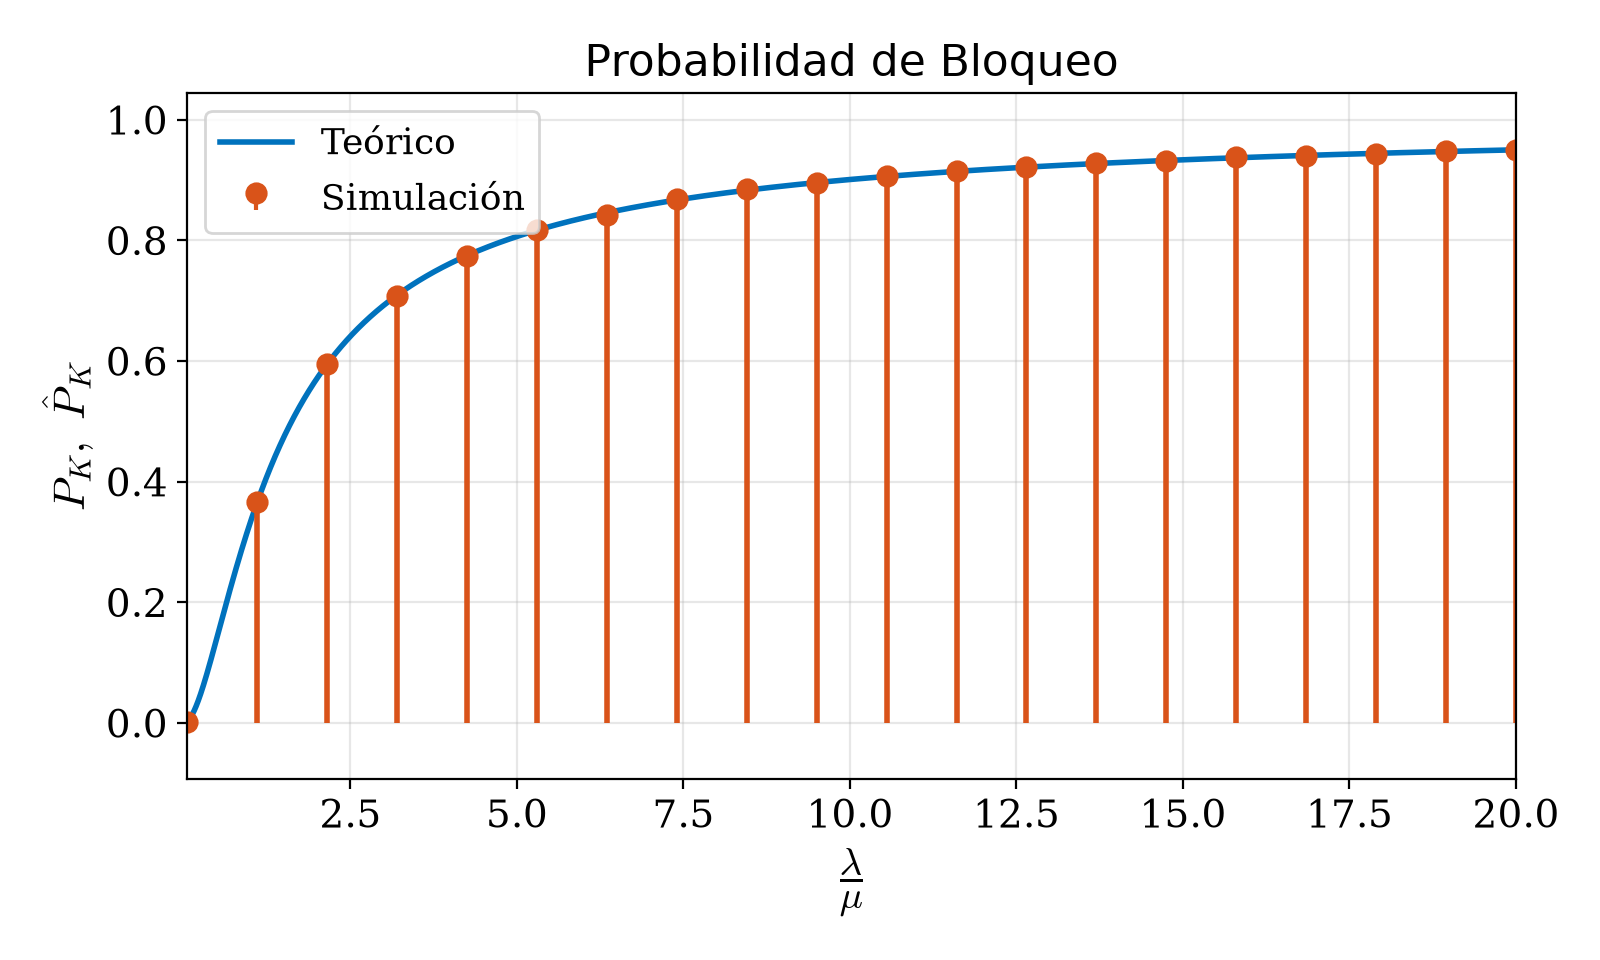
\includegraphics[width=\linewidth]{actividad3_100000.png}
    \caption{$10^5$ usuarios}
\end{subfigure}

\begin{subfigure}{0.62\textwidth}
    \centering
    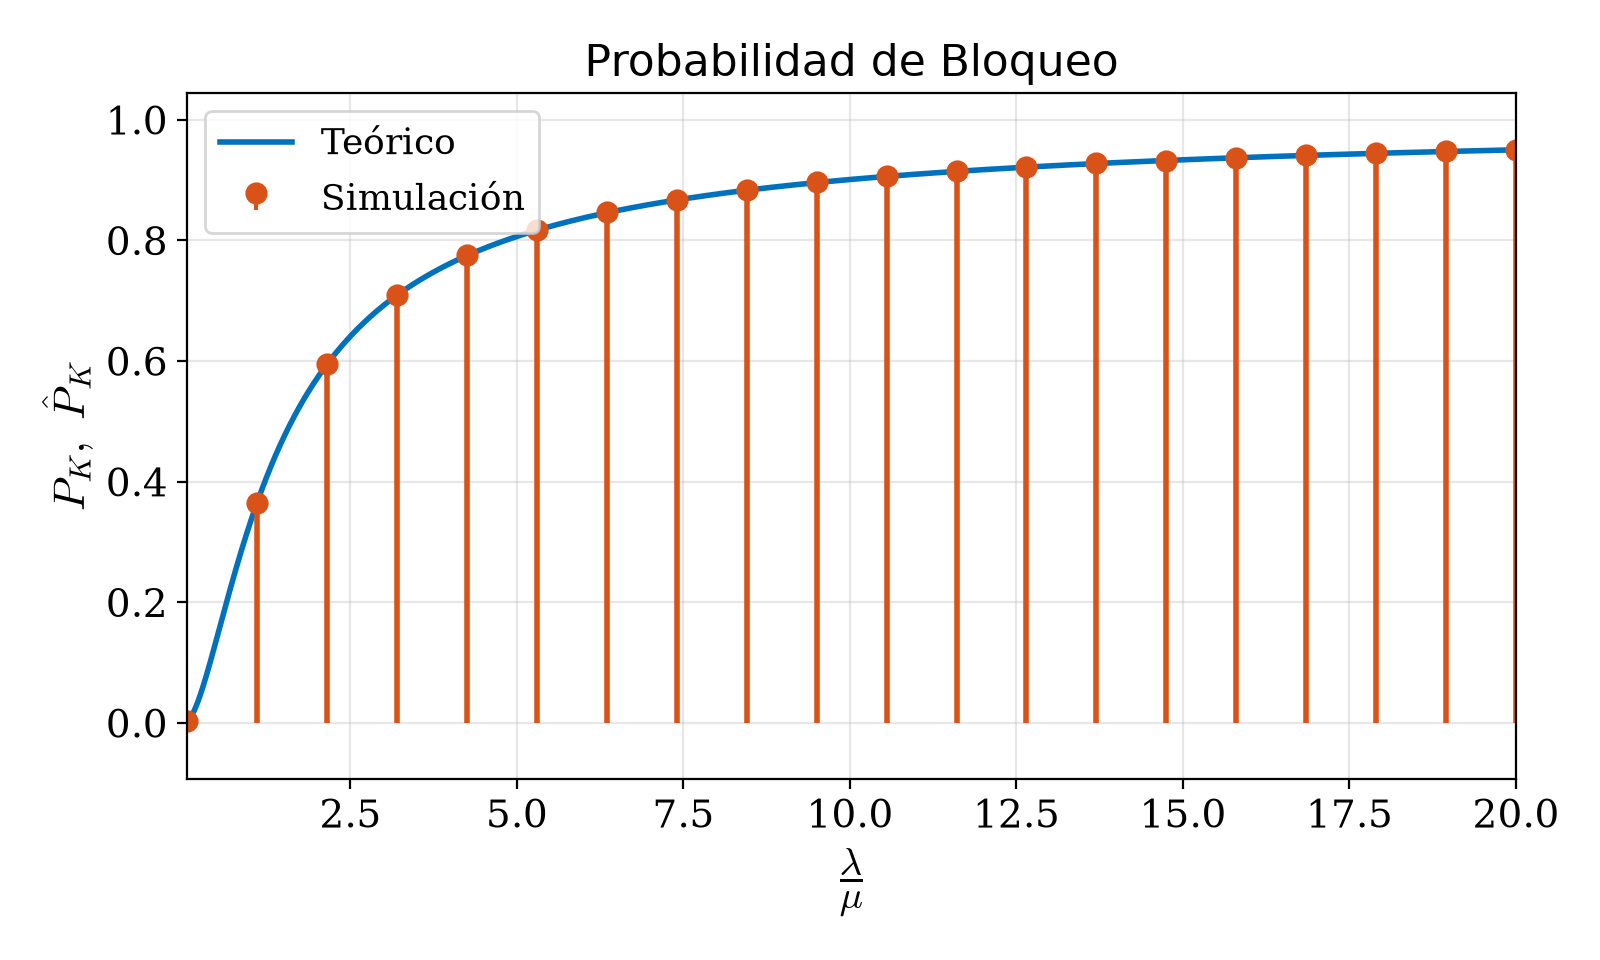
\includegraphics[width=\linewidth]{actividad3_1000000.png}
    \caption{$10^6$ usuarios}
\end{subfigure}

\begin{subfigure}{0.62\textwidth}
    \centering
    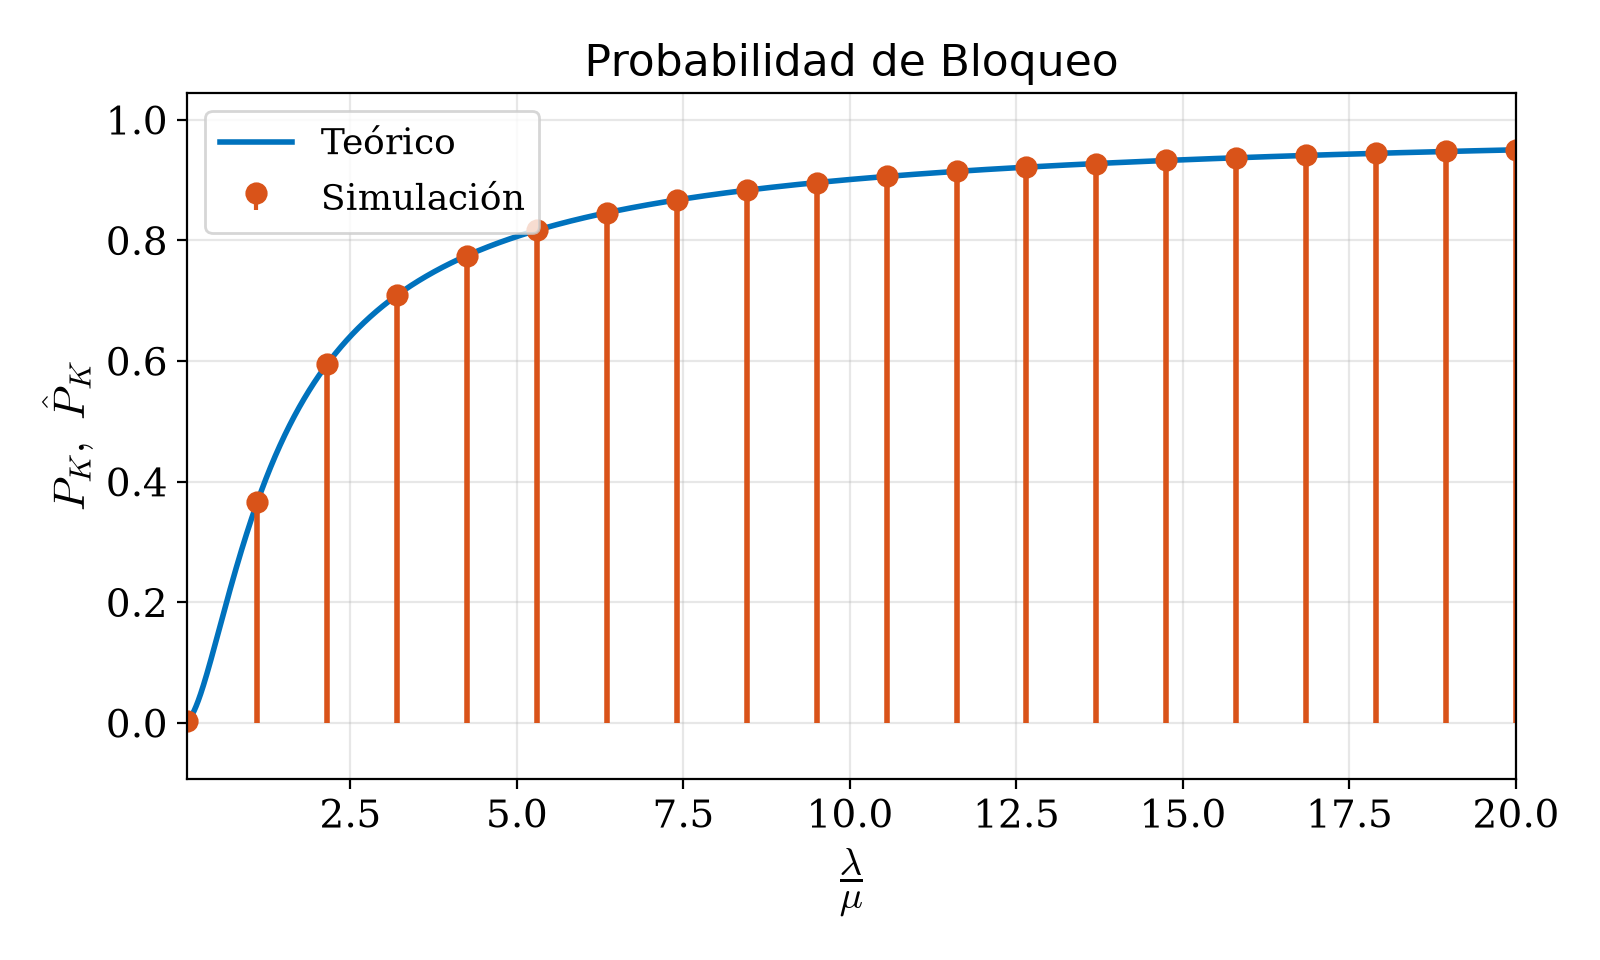
\includegraphics[width=\linewidth]{actividad3_10000000.png}
    \caption{$10^7$ usuarios}
\end{subfigure}
\caption{Probabilidad de bloqueo de la cola M/M/1/K con $K=2$ versus $A=\lambda/\mu$: valor teórico (línea) y estimación por simulación (puntos).}
\label{fig:actividad3}
\end{figure}

A simple vista las tres gráficas son iguales: en todos los casos los puntos simulados caen sobre la curva teórica. Las diferencias se aprecian en los valores numéricos. El Cuadro~\ref{tab:actividad3} compara algunos de ellos con el valor teórico, y el Cuadro~\ref{tab:errores} resume la diferencia entre la simulación y la teoría en los 20 valores de $A$.

\begin{table}[!htbp]
\centering
\begin{tabular}{c c c c c}
\hline
$A$ & $\hat{P}_K$ ($10^5$ usuarios) & $\hat{P}_K$ ($10^6$ usuarios) & $\hat{P}_K$ ($10^7$ usuarios) & $P_K$ (teórico) \\
\hline
1,10  & 0,3661 & 0,3646 & 0,3656 & 0,3656 \\
2,15  & 0,5958 & 0,5944 & 0,5946 & 0,5947 \\
6,35  & 0,8420 & 0,8464 & 0,8460 & 0,8458 \\
10,55 & 0,9065 & 0,9059 & 0,9060 & 0,9060 \\
20,00 & 0,9502 & 0,9499 & 0,9501 & 0,9501 \\
\hline
\end{tabular}
\caption{Probabilidad de bloqueo simulada y teórica para $K=2$ en algunos valores de $A$.}
\label{tab:actividad3}
\end{table}

\begin{table}[!htbp]
\centering
\begin{tabular}{c c c}
\hline
Usuarios & $\max\left|\hat{P}_K-P_K\right|$ & Promedio de $\left|\hat{P}_K-P_K\right|$ \\
\hline
$10^5$ & 0,00379 & 0,00074 \\
$10^6$ & 0,00097 & 0,00028 \\
$10^7$ & 0,00025 & 0,00009 \\
\hline
\end{tabular}
\caption{Diferencia entre la simulación y el valor teórico en los 20 valores de $A$.}
\label{tab:errores}
\end{table}

\subsection{Análisis de los resultados}

\begin{itemize}
    \item \textbf{Coincidencia con la teoría.} En todo el intervalo de $A$, tanto para $A<1$ como para $A>1$, los valores simulados coinciden con la curva teórica. Esto valida la función \texttt{mm1k}: la simulación reproduce el resultado analítico de la Actividad 1, obtenido por un método completamente distinto.
    \item \textbf{Ley de los grandes números.} La mayor diferencia pasa de $0{,}00379$ con $10^5$ usuarios a $0{,}00097$ con $10^6$ y a $0{,}00025$ con $10^7$. Cada vez que la cantidad de usuarios se multiplica por 10, el error se reduce casi cuatro veces. Las diferencias que quedan se deben a que cada simulación usa una cantidad finita de usuarios, no a un error en la lógica de la cola.
    \item \textbf{Tráfico bajo.} Para $A$ pequeño casi ningún usuario se bloquea: con $A=0{,}05$, $P_K=0{,}0024$. Los usuarios llegan con poca frecuencia comparada con la rapidez del servidor, y casi siempre encuentran el sistema con espacio.
    \item \textbf{Crecimiento de la probabilidad de bloqueo.} La probabilidad de bloqueo crece rápidamente cuando $A$ aumenta desde cero: en $A=1$, cuando llegan en promedio tantos usuarios como el servidor puede atender, ya se bloquea uno de cada tres ($P_K=1/(K+1)=1/3$), y en $A=5$ se bloquea el 81\%. Después el crecimiento es más lento.
    \item \textbf{Tráfico alto.} Con $K=2$, la probabilidad de bloqueo se puede escribir como $P_K=A^2/(A^2+A+1)$, que tiende a 1 cuando $A\to\infty$. En $A=10$ se bloquea el 90\% de los usuarios y en $A=20$ el 95\%: llegan muchos más usuarios de los que el servidor puede atender, y la capacidad de la línea de espera, de un solo puesto, no alcanza para recibirlos.
    \item \textbf{Simulación con $A\geq1$.} A diferencia de la M/M/1, cuya serie solo converge con $A<1$, la cola M/M/1/K se simuló sin problema hasta $A=20$. En lugar de que la línea de espera crezca sin límite, el exceso de usuarios se convierte en usuarios bloqueados.
\end{itemize}

\section{Actividad 4}

Utilicen la función \texttt{superfuncion} (que hará parte de una tarea futura), para generar cuatro funciones asociadas al conjunto de datos suministrados en clase. Muestren evidencias de la validez de sus funciones (comparación de las gráficas de las distribuciones de los datos y gráficas qqplot, por ejemplo).

\subsection{Datos}

Los cuatro archivos corresponden a trazas de tráfico Ethernet medidas en los laboratorios de Bellcore en 1989 \autocite{leland1994}. Cada archivo tiene $10^6$ filas y dos columnas: el instante de llegada de cada paquete, en segundos, y su tamaño en bytes. Los tiempos entre arribos se obtienen como la diferencia entre instantes consecutivos de la primera columna, de modo que cada muestra tiene $999\,999$ valores. El Cuadro~\ref{tab:datos} resume cada muestra.

\begin{table}[!htbp]
\centering
{\small\setlength{\tabcolsep}{4pt}
\begin{tabular}{l l c c c c c}
\hline
Archivo & Función & Duración & Media & Mediana & $\sigma/\text{media}$ & $\hat{\lambda}=1/\text{media}$ \\
 & & (h) & (ms) & (ms) & & (paquetes/s) \\
\hline
\texttt{BCpAug89.TL}    & \texttt{agostornd}      & 0,87 & 3,143 & 1,956 & 1,80 & 318,2 \\
\texttt{BCpOct89.TL}    & \texttt{octubrernd}     & 0,49 & 1,760 & 1,032 & 1,82 & 568,3 \\
\texttt{BCOct89Ext.TL}  & \texttt{octubreextrnd}  & 34,1 & 122,8 & 19,31 & 4,03 & 8,1 \\
\texttt{BCOct89Ext4.TL} & \texttt{octubreext4rnd} & 21,1 & 75,94 & 5,168 & 3,90 & 13,2 \\
\hline
\end{tabular}}
\caption{Tiempos entre arribos de los cuatro archivos de datos.}
\label{tab:datos}
\end{table}

En una distribución exponencial la desviación estándar es igual a la media, es decir, $\sigma/\text{media}=1$, y la mediana vale $\ln 2/\lambda\approx 0{,}69$ veces la media. En las cuatro muestras la desviación es entre 1,8 y 4 veces la media, y la mediana es mucho menor que la media. Por lo tanto, los tiempos entre arribos reales no son exponenciales, y para generarlos no sirve \texttt{exprnd}: se necesita un generador construido a partir de los propios datos.

\subsection{Fundamentos: pdf, CDF y función cuantil}

\textbf{pdf y CDF.} Una variable aleatoria continua $X$ se describe con su función de densidad de probabilidad, $f_X(x)$, o con su función de distribución acumulativa,
\[
F_X(x)=P[X\leq x]=\int_{-\infty}^{x}f_X(u)\,du,\qquad f_X(x)=\frac{dF_X(x)}{dx}.
\]
$F_X$ es no decreciente, empieza en 0 y llega a 1.

\textbf{Estimación a partir de una muestra.} La función \texttt{pdfcdfcontinua} divide el intervalo de observación $[a,b]$ con $m=\lfloor\sqrt{n}\rfloor$ puntos igualmente espaciados $x_1,\dots,x_m$, separados $\Delta x$, y cuenta cuántos de los $n$ datos caen en cada intervalo $[x_j,x_{j+1})$, digamos $n_j$. Las estimaciones son
\[
\hat{f}_X(x_j)=\frac{n_j}{n\,\Delta x},\qquad \hat{F}_X(x_j)=\sum_{i=1}^{j}\frac{n_i}{n}.
\]
Los datos mayores que $b$ no se cuentan, así que $\hat{F}_X(b)$ es la fracción de la muestra que queda dentro del intervalo. Por eso el intervalo se escoge de modo que la CDF estimada llegue cerca de 1 y, al mismo tiempo, se vea el detalle de la zona donde se concentra la probabilidad.

\textbf{Función cuantil.} Es la inversa de la CDF:
\[
Q_X(p):=F_X^{-1}(p),\qquad 0\leq p\leq 1.
\]
Si $F_X$ tiene tramos planos, se toma $Q_X(p)=\min\{x: F_X(x)\geq p\}$.

\textbf{Método de la transformación inversa.} Si $U\sim\mathcal{U}(0,1)$, entonces $X=Q_X(U)$ tiene CDF $F_X$, porque
\[
P[Q_X(U)\leq x]=P[U\leq F_X(x)]=F_X(x).
\]
Así, para generar números aleatorios con cualquier distribución basta un generador uniforme y la función cuantil.

\textbf{Función cuantil empírica y \texttt{superfuncion}.} Los datos reales no tienen una función cuantil analítica, así que se estima numéricamente. \texttt{superfuncion} calcula con \texttt{quantile} los cuantiles de la muestra en $N=10^5$ probabilidades igualmente espaciadas entre 0 y 1, y escribe un archivo \texttt{.m} con una función que los guarda. Cada vez que se llama, la función escoge al azar, con \texttt{randi}, una de esas $N$ posiciones y retorna el cuantil correspondiente. Es el método de la transformación inversa con $p$ uniforme sobre una malla de $N$ puntos. Dos consecuencias: los números generados quedan entre el mínimo y el máximo de la muestra, y cada punto de la malla representa una probabilidad de $1/(N-1)\approx 10^{-5}$.

\textbf{Gráfica Q-Q.} La función \texttt{qqplot(x,y)} grafica los cuantiles de una muestra contra los de la otra, $\bigl(\hat{Q}_x(p),\hat{Q}_y(p)\bigr)$, y traza en rojo la recta que une los puntos del primer y el tercer cuartil. Si las dos muestras tienen la misma distribución, los puntos quedan sobre la recta $y=x$. Donde los puntos están muy juntos hay mucha probabilidad; los puntos aislados corresponden a regiones de baja probabilidad, y es normal que en ellas se separen un poco de la recta.

\subsection{Procedimiento}

Se utilizó el código guía de la Actividad 4 presentado en clase, repetido para los cuatro archivos. Para cada uno:

\begin{enumerate}
    \item Se cargan los datos y se calculan los tiempos entre arribos con \texttt{diff}.
    \item Se estiman la pdf y la CDF de la muestra con \texttt{pdfcdfcontinua}, en el intervalo de observación del Cuadro~\ref{tab:intervalos}.
    \item Se codifica el generador con \texttt{superfuncion}, con un nombre distinto para cada archivo.
    \item Se generan $10^6$ números con la función codificada y se estiman su pdf y su CDF en el mismo intervalo. Siguiendo la recomendación de clase, las estimaciones se superponen a las de la muestra para que las diferencias se noten.
    \item Se grafica la Q-Q de los números generados (eje x) contra la muestra (eje y) con \texttt{qqplot}.
    \item Se comparan la media, la mediana, la desviación estándar y la mayor diferencia entre las dos CDF estimadas,
    \[
    D=\max_j\bigl|\hat{F}_{\text{muestra}}(x_j)-\hat{F}_{\text{generada}}(x_j)\bigr|.
    \]
\end{enumerate}

\begin{table}[!htbp]
\centering
\begin{tabular}{l c c}
\hline
Archivo & Intervalo de observación (s) & $\hat{F}_X(b)$ \\
\hline
\texttt{BCpAug89.TL}    & $[-0{,}001;\ 0{,}006]$  & 0,931 \\
\texttt{BCpOct89.TL}    & $[-0{,}0005;\ 0{,}005]$ & 0,955 \\
\texttt{BCOct89Ext.TL}  & $[-0{,}05;\ 0{,}5]$     & 0,958 \\
\texttt{BCOct89Ext4.TL} & $[-0{,}03;\ 0{,}3]$     & 0,950 \\
\hline
\end{tabular}
\caption{Intervalos de observación. El de agosto es el usado en clase; los demás se escogieron con el mismo criterio.}
\label{tab:intervalos}
\end{table}

El código completo se encuentra en el Anexo~\ref{anexo:actividad4}.

\subsection{Resultados}

Las Figuras~\ref{fig:a4agosto} a~\ref{fig:a4ext4} muestran, para cada archivo, la pdf y la CDF de la muestra y de la función codificada, y la gráfica Q-Q. El Cuadro~\ref{tab:comparacion} resume la comparación numérica.

\newcommand{\figuraactividadcuatro}[3]{%
\begin{figure}[!htbp]
\centering
\begin{subfigure}{0.52\textwidth}
    \centering
    \includegraphics[width=\linewidth]{actividad4_pdfcdf_#1.png}
    \caption{pdf y CDF estimadas.}
\end{subfigure}%
\hfill
\begin{subfigure}{0.44\textwidth}
    \centering
    \includegraphics[width=\linewidth]{actividad4_qq_#1.png}
    \caption{Gráfica Q-Q: función (eje x) y muestra (eje y).}
\end{subfigure}
\caption{Validación de la función \texttt{#1}, generada a partir de \texttt{#2}.}
\label{#3}
\end{figure}}

\figuraactividadcuatro{agostornd}{BCpAug89.TL}{fig:a4agosto}
\figuraactividadcuatro{octubrernd}{BCpOct89.TL}{fig:a4octubre}
\figuraactividadcuatro{octubreextrnd}{BCOct89Ext.TL}{fig:a4ext}
\figuraactividadcuatro{octubreext4rnd}{BCOct89Ext4.TL}{fig:a4ext4}

\begin{table}[!htbp]
\centering
{\small\setlength{\tabcolsep}{4pt}
\begin{tabular}{l c c c c c c c}
\hline
 & \multicolumn{2}{c}{Media (ms)} & \multicolumn{2}{c}{Mediana (ms)} & \multicolumn{2}{c}{Desviación (ms)} & \\
Función & Muestra & Generada & Muestra & Generada & Muestra & Generada & $D$ \\
\hline
\texttt{agostornd}      & 3,143 & 3,145 & 1,956 & 1,956 & 5,643 & 5,731 & 0,0010 \\
\texttt{octubrernd}     & 1,760 & 1,760 & 1,032 & 1,032 & 3,199 & 3,223 & 0,0006 \\
\texttt{octubreextrnd}  & 122,8 & 122,3 & 19,31 & 19,26 & 494,5 & 491,5 & 0,0007 \\
\texttt{octubreext4rnd} & 75,94 & 75,31 & 5,168 & 5,160 & 295,9 & 293,7 & 0,0007 \\
\hline
\end{tabular}}
\caption{Comparación entre cada muestra y $10^6$ números generados con su función.}
\label{tab:comparacion}
\end{table}

\subsection{Análisis de los resultados}

\begin{itemize}
    \item \textbf{Agosto.} La pdf no se parece a la de una exponencial, que es decreciente desde $t=0$: tiene varios picos angostos, cerca de 0,07; 0,14; 0,9; 1,3 y 1,9~ms, y dos zonas más anchas alrededor de 3 y 4~ms. El 93\% de los tiempos es menor que 6~ms. Las curvas de la muestra y de \texttt{agostornd} se superponen, incluidos los picos. La gráfica Q-Q es una recta de pendiente 1 hasta unos 0,14~s; por encima de ese valor solo hay puntos aislados, pues apenas 7 de los $999\,999$ tiempos superan 0,2~s.
    \item \textbf{Octubre.} La probabilidad está aún más concentrada: el 11,7\% de los tiempos está entre 0,90 y 0,93~ms, lo que produce el pico principal de la pdf y el salto de la CDF en ese valor. El 95,5\% de los datos es menor que 5~ms. Las curvas coinciden y la gráfica Q-Q es recta hasta unos 0,09~s.
    \item \textbf{Octubre extendido y extendido 4.} Son mediciones mucho más largas, de 34 y 21 horas, con tiempos más largos y más variables: la desviación es unas 4 veces la media. La probabilidad se concentra cerca de cero, la mediana es de 19 y 5~ms, y la cola se extiende hasta 10 y 8~s. Las curvas coinciden; la gráfica Q-Q de \texttt{octubreextrnd} es recta en todo el rango, y la de \texttt{octubreext4rnd} hasta unos 5~s.
    \item \textbf{Comparación numérica.} Las medianas coinciden casi exactamente, las medias difieren menos del 1\% y las desviaciones menos del 2\%. La mayor diferencia entre las CDF estimadas es de 0,001 o menos. Las diferencias en la media y la desviación se deben a la cola derecha, que es donde más pesa cada dato.
    \item \textbf{Puntos que se separan de la recta.} En las cuatro gráficas Q-Q los puntos que se alejan de la recta están por encima del percentil 99,9, es decir, en el 0,1\% de los datos con menor probabilidad. La causa es la malla de \texttt{superfuncion}: en esa cola los cuantiles consecutivos de la malla están muy separados, y la función solo puede generar esos pocos valores, por lo que en la gráfica aparecen columnas verticales de puntos. Como esa región tiene muy baja probabilidad, no afecta la aproximación de la distribución.
\end{itemize}

En conclusión, las cuatro funciones reproducen la distribución de los tiempos entre arribos reales: las pdf y CDF estimadas se superponen, las gráficas Q-Q son rectas en la región donde se concentra la probabilidad y los estadísticos coinciden. Como estos tiempos no son exponenciales, en la Actividad 5 no se espera que la probabilidad de bloqueo simulada con estas funciones coincida con el valor teórico de la M/M/1/K.

\section{Actividad 5}
 
Realicen la simulación de la cola asignada variando $A=\lambda/\mu$. Consideren que los elementos del vector de tiempos entre arribos consecutivos, se obtienen con cada una de las cuatro funciones de la cuarta actividad (para cada función consideren que el parámetro $\lambda$, se estima con el inverso multiplicativo de la media aritmética de los elementos del vector generado con cada una de las cuatro funciones: $\lambda\approx 1/\overline{T}_{arribo}$), y que los elementos del vector de tiempos de servicio se distribuyen exponencialmente, con parámetro $\mu$. Como resultado principal, realicen las cuatro gráficas de la medida de desempeño versus $A$. Comparen los resultados de simulación con el valor teórico (para distribuciones exponenciales) de la medida de desempeño.
 
\subsection{Qué cambia respecto a la Actividad 3}
 
En la Actividad 3 los dos tiempos eran exponenciales, así que la cola era una M/M/1/K y la probabilidad de bloqueo tenía una fórmula exacta. Ahora los tiempos entre arribos siguen la distribución de los datos de Bellcore, que no es exponencial (Cuadro~\ref{tab:datos}), mientras que los tiempos de servicio siguen siendo exponenciales. La cola deja de ser M/M/1/K y pasa a ser una G/M/1/K, para la cual no se tiene la fórmula de la Actividad 1.
 
Esto no obliga a cambiar el simulador. Igual que \texttt{xx1}, la función \texttt{mm1k} solo usa los vectores \texttt{tea} y \texttt{tds} y no depende de su distribución, así que se usa tal cual. Lo que sí cambia es el papel de la curva teórica: ya no es el valor que la simulación debe reproducir, sino la referencia que dice cuánto se bloquearía si los arribos fueran exponenciales con la misma tasa media.
 
\subsection{Valor teórico de referencia}
 
Con $K=5$, la probabilidad de bloqueo para arribos y servicios exponenciales (Actividad 1) es
\[
P_5(A)=\frac{(1-A)A^{5}}{1-A^{6}},\qquad A\neq 1,\qquad\qquad P_5(1)=\frac{1}{6}.
\]
Esta curva solo describe el caso exponencial. Que las simulaciones no caigan sobre ella no indica un error en \texttt{mm1k}, ya validada en las Actividades 2 y 3: indica que la distribución de los tiempos entre arribos influye en el bloqueo, aunque $\lambda$ y $\mu$ sean los mismos.
 
\subsection{Procedimiento}
 
Se utilizó el código de la Actividad 3 con los siguientes cambios:
 
\begin{enumerate}
    \item \textbf{Tiempos entre arribos.} Para cada una de las funciones \texttt{agostornd}, \texttt{octubrernd}, \texttt{octubreextrnd} y \texttt{octubreext4rnd} se genera un vector de $10^6$ tiempos entre arribos. Se usa el mismo vector para todos los valores de $A$, de modo que las diferencias entre un punto y otro de la gráfica se deban solo a $A$ y a los tiempos de servicio.
    \item \textbf{Estimación de $\lambda$.} Siguiendo el enunciado, $\hat{\lambda}=1/\overline{T}_{arribo}$, con $\overline{T}_{arribo}$ la media aritmética del vector generado con cada función. Queda en paquetes por segundo, porque los datos están en segundos.
    \item \textbf{Variación de $A$.} A diferencia de la Actividad 3, aquí $\lambda$ no se puede escoger: lo fijan los datos. Por eso lo que se modifica es $\mu$, con $\mu=\hat{\lambda}/A$.
    \item \textbf{Tiempos de servicio.} Para cada valor de $A$ se generan $10^6$ tiempos de servicio con \texttt{exprnd}, con media $1/\mu$.
    \item \textbf{Capacidad y rango de $A$.} Se usa $K=5$: un usuario en servicio y como máximo cuatro en la línea de espera. Se toman 40 valores de $A$ igualmente espaciados entre $0{,}05$ y $4K=20$. Con $K=5$ el bloqueo teórico ya vale $0{,}95$ en $A=20$, el mismo valor con el que terminó la gráfica de la Actividad 3, y hay más puntos que en aquella actividad porque ahora interesa ver bien la zona donde la curva cambia rápido.
    \item \textbf{Estimación del bloqueo.} Para cada $A$ se calcula $\hat{P}_K$ con \texttt{mm1k}. Los resultados se grafican con \texttt{superstem} sobre la curva teórica de la Actividad 3 (\texttt{superplot}), una gráfica por función.
\end{enumerate}
 
El código completo se encuentra en el Anexo~\ref{anexo:actividad5}.
 
\subsection{Cota para tráfico alto}
 
Hay un resultado que no depende de la distribución de los arribos. En el largo plazo, la tasa de usuarios que entran al sistema, $\lambda(1-P_K)$, es igual a la tasa de usuarios atendidos, y esa tasa no puede superar la capacidad del servidor, $\mu$. Entonces
\[
\lambda(1-P_K)\leq\mu\;\Rightarrow\;P_K\geq 1-\frac{1}{A}.
\]
Para $A=20$, cualquier cola de este tipo bloquea al menos el 95\% de los usuarios, y la curva exponencial queda justo en esa cota. Por lo tanto, para $A$ grande las cuatro simulaciones tienen que quedar pegadas a la curva teórica sin importar los datos; las diferencias deben aparecer en tráfico bajo y moderado.
 
\subsection{Resultados}
 
Las Figuras~\ref{fig:a5agostornd} a~\ref{fig:a5octubreext4rnd} muestran, para cada función, la probabilidad de bloqueo simulada y la teórica para arribos exponenciales. El Cuadro~\ref{tab:a5resumen} resume cada simulación.
 
\newcommand{\figuraactividadcinco}[2]{%
\begin{figure}[!htbp]
\centering
\IfFileExists{figuras/actividad5_#1.png}{\includegraphics[width=0.72\linewidth]{actividad5_#1.png}}{\fbox{\parbox{0.6\linewidth}{\centering Falta la figura \texttt{figuras/actividad5\_#1.png}}}}
\caption{Probabilidad de bloqueo con $K=5$ versus $A=\lambda/\mu$, con arribos generados por \texttt{#1} (a partir de \texttt{#2}): valor teórico para arribos exponenciales (línea) y simulación (puntos).}
\label{fig:a5#1}
\end{figure}}
 
\figuraactividadcinco{agostornd}{BCpAug89.TL}
\figuraactividadcinco{octubrernd}{BCpOct89.TL}
\figuraactividadcinco{octubreextrnd}{BCOct89Ext.TL}
\figuraactividadcinco{octubreext4rnd}{BCOct89Ext4.TL}
 
% COMPLETAR: llenar el cuadro con la salida de "resumen" de actividad5.m
% (columnas: lambda estimada, desviación/media, mayor diferencia con el teórico).
\begin{table}[!htbp]
\centering
\begin{tabular}{l c c c}
\hline
Función & $\hat{\lambda}$ (paquetes/s) & $\sigma/\text{media}$ & $\max\left|\hat{P}_K-P_K^{\text{exp}}\right|$ \\
\hline
\texttt{agostornd}      & \textbf{?} & \textbf{?} & \textbf{?} \\
\texttt{octubrernd}     & \textbf{?} & \textbf{?} & \textbf{?} \\
\texttt{octubreextrnd}  & \textbf{?} & \textbf{?} & \textbf{?} \\
\texttt{octubreext4rnd} & \textbf{?} & \textbf{?} & \textbf{?} \\
\hline
\end{tabular}
\caption{Resumen de las simulaciones con $K=5$ y $10^6$ usuarios.}
\label{tab:a5resumen}
\end{table}
 
\subsection{Análisis de los resultados}
% COMPLETAR: los puntos entre corchetes dependen de lo que muestren las figuras.
\begin{itemize}
    \item \textbf{Las simulaciones no siguen la curva exponencial.} Las cuatro funciones tienen $\sigma/\text{media}$ entre 1,8 y 4, y la exponencial tiene 1. [Describir en qué zona de $A$ los puntos quedan por encima o por debajo de la curva teórica y cuánto se separan.]
    \item \textbf{Efecto de la variabilidad.} Con la misma tasa media de arribo, los tiempos entre arribos más dispersos agrupan a los usuarios en ráfagas y cambian cuántos encuentran el sistema lleno. [Comparar los archivos de agosto y octubre ($\sigma/\text{media}\approx 1{,}8$) con los dos archivos \texttt{Ext} ($\approx 4$): ¿la separación crece con la variabilidad?]
    \item \textbf{Tráfico alto.} Por la cota $P_K\geq 1-1/A$, todas las curvas se acercan a 1 y a la curva teórica cuando $A$ crece. [Confirmar en las figuras desde qué valor de $A$ ya no se distinguen.]
    \item \textbf{Independencia de los arribos generados.} \texttt{superfuncion} reproduce la distribución de los tiempos entre arribos, pero cada número se escoge de forma independiente de los anteriores. El tráfico de Bellcore medido por Leland et al.~\autocite{leland1994} tiene dependencia entre arribos consecutivos (es autosimilar), y esa dependencia se pierde al generar los vectores. Por eso estas simulaciones capturan el efecto de la distribución de los tiempos, pero no el de su orden, y el bloqueo del tráfico real probablemente sea mayor.
    \item \textbf{Efecto de $K$.} [Opcional: comparar con la Actividad 3 ($K=2$): con más capacidad el bloqueo teórico en tráfico bajo es mucho menor, y la separación entre simulación y teoría se nota más en términos relativos.]
\end{itemize}
 

\section{Conclusiones}

\printbibliography[title={Referencias}]

\newpage
\appendix
\renewcommand{\lstlistingname}{Código}

\section{Código de la función \texttt{mm1k}}\label{anexo:mm1k}

\IfFileExists{codigos/mm1k.m}{%
\lstinputlisting[caption={Función \texttt{mm1k} para simular la cola M/M/1/K.}]{codigos/mm1k.m}%
}{\textbf{Falta subir el archivo codigos/mm1k.m al proyecto.}}

\section{Código de la prueba y la validación de la función \texttt{mm1k}}\label{anexo:pruebas}

\begin{lstlisting}[caption={Prueba de \texttt{mm1k} con los vectores de clase.}]
tea = [1,2,3,7,2,3,8,0,5];
tds = [9,1,4,1,1,5,3,8,2];
Pk = mm1k(tea,tds,2)   % Pk = 0.1111
\end{lstlisting}

\begin{lstlisting}[caption={Validación de \texttt{mm1k} con tiempos exponenciales.}]
mu = 4;
A = 0.5;
lambda = A*mu;
K = 2;
usuarios = 1000000;
tea = exprnd(1/lambda,1,usuarios);
tds = exprnd(1/mu,1,usuarios);
Pk = mm1k(tea,tds,K,0)                 % no muestra los vectores
Pkteorico = (1-A)*A^K/(1-A^(K+1))
\end{lstlisting}

\section{Código de la simulación de la Actividad 3}\label{anexo:actividad3}

\IfFileExists{codigos/actividad3.m}{%
\lstinputlisting[caption={Simulación de la cola M/M/1/K variando $A=\lambda/\mu$.}]{codigos/actividad3.m}%
}{\textbf{Falta subir el archivo codigos/actividad3.m al proyecto.}}

\section{Código de la Actividad 4}\label{anexo:actividad4}

\IfFileExists{codigos/actividad4.m}{%
\lstinputlisting[caption={Generación y validación de las cuatro funciones con \texttt{superfuncion}.}]{codigos/actividad4.m}%
}{\textbf{Falta subir el archivo codigos/actividad4.m al proyecto.}}

\section{Código de la simulación de la Actividad 5}\label{anexo:actividad5}

\IfFileExists{codigos/actividad5.m}{%
\lstinputlisting[caption={Simulación de la cola con arribos generados por las cuatro funciones de la Actividad 4.}]{codigos/actividad5.m}%
}{\textbf{Falta subir el archivo codigos/actividad5.m al proyecto.}}

\end{document}
